% ROZDZIAŁ 29 -- podstawy geometrycznej teorii miary
\chapter[Prostowalność i zbiory o skończonym obwodzie]{Zbiory prostowalne, funkcje BV i zbiory o skończonym obwodzie}
\label{ch:geometric-measure-29}

\section{Cel i zakres teorii}
W geometrii różniczkowej badaliśmy gładkie podrozmaitości, ich
metryki indukowane oraz normalne. W tym rozdziale będziemy mierzyć
również brzegi zbiorów, które mają narożniki, pęknięcia lub
nieregularności i nie są podrozmaitościami. Zamiast zakładać
istnienie klasycznej normalnej w każdym punkcie, zdefiniujemy ją
\emph{miarowo}. Przygotujemy w ten sposób język geometrycznej
teorii miary, teorii wariacyjnej i równań różniczkowych cząstkowych.

Pracujemy na $\mathbb R^n$, gdzie $n\ge1$, z miarą Lebesgue'a
$\lambda_n$ i miarami Hausdorffa $\mathcal H^s$
z Rozdziału~\ref{ch:hausdorff-26}; dla wymiarów
całkowitych stosujemy dokładnie kalibrację
z Uwagi~\ref{rem:hausdorff-convention-26}.
W szczególności $\mathcal H^{n-1}$ ma tę samą
normalizację co we wzorze area z
Rozdziału~\ref{ch:area-coarea-28}, a gdy $n=1$,
$\mathcal H^0$ jest miarą liczącą. Oznaczenie $\chi_E$ oznacza
funkcję charakterystyczną $E$. Wszystkie przestrzenie $L^1$
są przestrzeniami klas funkcji równych prawie wszędzie.
Stosujemy przy tym konwencję dystrybucyjną
$\langle D_i u,\varphi\rangle=-\int_{\mathbb R^n}u(x)
\partial_i\varphi(x)\,\mathrm d\lambda_n(x)$ dla
$\varphi\in C_c^1(\mathbb R^n)$.

\section{Prostowalność: co pozostaje z gładkiej powierzchni?}
\begin{definicja}[Zbiory przeliczalnie prostowalne]
\label{def:rectifiable-29}
Niech $1\le k\le n$. Zbiór $E\subseteq\mathbb R^n$ nazywamy
\emph{przeliczalnie $k$-prostowalnym}, jeśli istnieją
zbiory $A_j\subseteq\mathbb R^k$ oraz odwzorowania
Lipschitzowskie $f_j:A_j\to\mathbb R^n$, $j\in\mathbb N$,
takie że
\[
 \mathcal H^k\!\left(E\setminus\bigcup_{j=1}^\infty f_j(A_j)\right)=0.
\]
Mówimy, że $E$ jest \emph{$k$-prostowalny o skończonej mierze},
jeżeli dodatkowo $\mathcal H^k(E)<\infty$.
Zbiór $P\subseteq\mathbb R^n$ jest \emph{czysto
$k$-nieprostowalny}, gdy
$\mathcal H^k(P\cap f(A))=0$ dla każdego
$A\subseteq\mathbb R^k$ i każdego odwzorowania
Lipschitzowskiego $f:A\to\mathbb R^n$.
\end{definicja}

Dla $k=0$ zbiór nazywamy przeliczalnie $0$-prostowalnym,
jeśli jest przeliczalny; wtedy $\mathcal H^0$ jest miarą liczącą.

W tej definicji nie utożsamiamy prostowalności z topologiczną
gładkością. Funkcja Lipschitzowska może mieć punkty załamania,
a zbiór prostowalny może być przeliczalną sumą rozłącznych
fragmentów powierzchni. Warunek z miarą Hausdorffa pozwala
pominąć tylko zbiór $k$-wymiarowo zerowy, nie dowolny zbiór
mały w sensie miary $n$-wymiarowej.

\begin{przyklad}[Wykres z narożnikiem]
\label{ex:lip-graph-29}
Zbiór $E=\{(t,|t|):-1\le t\le1\}\subseteq\mathbb R^2$
jest $1$-prostowalny: to obraz przedziału przez odwzorowanie
$F(t)=(t,|t|)$, którego stała Lipschitza jest nie większa
niż $\sqrt2$. W punkcie $(0,0)$ nie jest on jednowymiarową
podrozmaitością klasy $C^1$. Mimo to $\mathcal H^1(E)$
jest skończona i dodatnia: rzut $E\to[-1,1]$ jest
$1$-Lipschitzowski, a odwzorowanie $F$ jest
$\sqrt2$-Lipschitzowskie, więc
$2\le\mathcal H^1(E)\le2\sqrt2$.
Złożenie dwóch odcinków daje nawet
$\mathcal H^1(E)=2\sqrt2$ na podstawie addytywności
miary na fragmentach przecinających się tylko w jednym punkcie.
\end{przyklad}

\begin{lemat}[Podstawowe własności prostowalności]
\label{lem:rectifiable-union-29}
Niech $1\le k\le n$. Wtedy:
\begin{enumerate}[label=(\roman*)]
\item przeliczalna suma zbiorów przeliczalnie
$k$-prostowalnych jest przeliczalnie $k$-prostowalna;
\item każdy podzbiór zbioru przeliczalnie
$k$-prostowalnego jest przeliczalnie $k$-prostowalny;
\item obraz zbioru przeliczalnie $k$-prostowalnego
przez odwzorowanie Lipschitzowskie określone na jego
otoczeniu jest przeliczalnie $k$-prostowalny.
\end{enumerate}
\end{lemat}
\begin{proof}
W (i) przestawiamy pary indeksów w jedną rodzinę
przeliczalną. W (ii) korzystamy z monotoniczności
miary zewnętrznej Hausdorffa: zbiór wyjątkowy
nowego podzbioru mieści się w zbiorze wyjątkowym
pierwotnego pokrycia. W (iii) ograniczamy każde $f_j$ do zbioru
$A_j' = \{x\in A_j:f_j(x)\in E\}$, tak aby złożenie
$G\circ f_j|_{A_j'}$ było określone. Jeśli $G$ ma stałą
Lipschitza $L$ w otoczeniu rozważanego zbioru,
to te złożenia są Lipschitzowskie, a obraz
wyjątkowego zbioru ma zerową miarę $\mathcal H^k$,
bo $\mathcal H^k(G(A))\le L^k\mathcal H^k(A)$.
Dla odwzorowania lokalnie Lipschitzowskiego rozbijamy
dziedzinę na przeliczalnie wiele obszarów, na których
jest ono Lipschitzowskie.
\end{proof}

\begin{uwaga}[Rozkład prostowalny -- granica argumentu elementarnego]
Przy założeniu $\mathcal H^k(E)<\infty$ istnieje rozkład
$E=R\,\dot\cup\,P$ (z dokładnością do zbiorów zerowych),
w którym $R$ jest przeliczalnie $k$-prostowalny,
a $P$ jest czysto $k$-nieprostowalny.
Jego dowód można oprzeć na maksymalizacji miary części
prostowalnej, ale w pełnej ogólności potrzebna jest
\emph{mierzalność obrazów borelowskich przez odwzorowania
Lipschitzowskie} (teoria zbiorów analitycznych).
Nie przedstawiamy tego argumentu jako samodzielnego dowodu:
w dalszej części wystarczą definicja prostowalności,
Lemat~\ref{lem:rectifiable-union-29} oraz jawne przykłady
wykresów i brzegów kawałkami gładkich.
\end{uwaga}

\section{Dystrybucyjna pochodna funkcji całkowalnej lokalnie}
\begin{definicja}[Wariacja funkcji]
\label{def:BV-variation-29}
Niech $\Omega\subseteq\mathbb R^n$ będzie otwarty,
a $u\in L^1_{\mathrm{loc}}(\Omega)$. Definiujemy
\[
 |Du|(\Omega)=\sup\left\{
 \int_\Omega u(x)\operatorname{div}\varphi(x)
   \,\mathrm d\lambda_n(x):
 \varphi\in C_c^1(\Omega;\mathbb R^n),\quad
 |\varphi(x)|\le1\ \text{dla wszystkich }x\in\Omega
 \right\}.
\]
Przez $BV(\Omega)$ oznaczamy przestrzeń
funkcji $u\in L^1(\Omega)$, dla których
$|Du|(\Omega)<\infty$. Normę definiujemy wzorem
$\|u\|_{BV}=\|u\|_{L^1}+|Du|(\Omega)$.
W zastosowaniach do obszarów nieograniczonych
wygodna jest również lokalna klasa $BV_{\mathrm{loc}}(\Omega)$:
na każdym $V\Subset\Omega$ funkcja ma skończoną
wariację $|Du|(V)$.
\end{definicja}

W definicji nie jest wymagane istnienie klasycznej
pochodnej $u$. Symbol $Du$ na początku oznacza
funkcjonał dystrybucyjny; dopiero niżej udowodnimy,
że przy skończonej wariacji reprezentuje go
wektorowa miara Radona.

\begin{lemat}[Wariacja gładkiej funkcji]
\label{lem:BV-smooth-29}
Jeżeli $u\in C^1(\Omega)\cap L^1_{\mathrm{loc}}(\Omega)$,
to
\[
 |Du|(\Omega)=\int_\Omega|\nabla u(x)|
 \,\mathrm d\lambda_n(x)\in[0,+\infty].
\]
\end{lemat}
\begin{proof}
Całkowanie przez części dla testów o zwartym nośniku
daje $\int_\Omega u\operatorname{div}\varphi\,\mathrm d\lambda_n=-\int_\Omega\nabla u\cdot\varphi\,\mathrm d\lambda_n$.
Z nierówności Cauchy'ego--Schwarza wynika
$|Du|(\Omega)\le\int_\Omega|\nabla u|\,\mathrm d\lambda_n$.
Dla nierówności odwrotnej ustalmy $K\Subset\Omega$
i $\varepsilon>0$. Na $K$ pole
$-\nabla u/(|\nabla u|+\varepsilon)$ jest ciągłe i ma normę
nie większą niż $1$. Aproksymujemy je jednostajnie na
$K$ przez pole $C_c^1(\Omega;\mathbb R^n)$ o normie
nieprzekraczającej $1$, mnożąc przez funkcję odcinającą
i ewentualnie przez czynnik bliski $1$.
Z definicji wariacji dostajemy
$|Du|(\Omega)\ge\int_K|\nabla u|^2/(|\nabla u|+\varepsilon)$.
Przez $\varepsilon\downarrow0$ i wyczerpanie $\Omega$
zbiorami zwartymi otrzymujemy przeciwną nierówność.
\end{proof}

Przez miarę wektorową o wartościach w $\mathbb R^n$
rozumiemy w tym miejscu przeliczalnie addytywną
w normie funkcję zbioru; ogólna definicja i teoria
wariacji takich miar znajduje się w
Rozdziale~\ref{ch:vector-measures-30}.

\begin{twierdzenie}[Pochodna $Du$ jako miara wektorowa]
\label{thm:BV-measure-29}
Niech $u\in L^1_{\mathrm{loc}}(\Omega)$ oraz
$|Du|(\Omega)<\infty$. Wtedy istnieje jedyna
skończona miara wektorowa $Du=(D_1u,\ldots,D_nu)$,
której współrzędne są skończonymi miarami ze znakiem,
i
\[
 \int_\Omega u(x)\operatorname{div}\varphi(x)
 \,\mathrm d\lambda_n(x)
 =-\int_\Omega\varphi(x)\cdot\mathrm dDu(x)
 \qquad(\varphi\in C_c^1(\Omega;\mathbb R^n)).
\]
Jej wariacja całkowita spełnia
$|Du|(\Omega)=\sup_{|\varphi|\le1}|
\int_\Omega \varphi\cdot\mathrm dDu|$,
gdzie supremum przebiega testy z definicji.
Jeżeli $u\in BV_{\mathrm{loc}}(\Omega)$,
analogicznie otrzymujemy lokalnie skończoną
wektorową miarę Radona.
\end{twierdzenie}
\begin{proof}
Oznaczmy przez $V=|Du|(\Omega)$ wartość supremum.
Dla każdego $i$ funkcjonał
$T_i(\psi)=-\int_\Omega u\partial_i\psi\,\mathrm d\lambda_n$
spełnia $|T_i(\psi)|\le V\|\psi\|_\infty$,
gdyż testujemy pole $\varphi=\psi e_i/\|\psi\|_\infty$
(zera nie wymagają osobnego przypadku). Funkcjonał ten
przedłuża się ciągle z $C_c^1(\Omega)$ do $C_0(\Omega)$:
przestrzeń testów jest gęsta dla normy supremum,
co wynika z konstrukcji funkcji odcinających i wygładzania.
Twierdzenie Riesza--Markowa--Kakutaniego
(Rozdział~\ref{ch:riesz-markov-21})
daje miarę ze znakiem $D_i u$. Złóżmy je w miarę wektorową
$Du=(D_iu)_i$, uzyskując podaną równość.

Aby określić dokładną wariację, przyjmijmy
$\mu=\sum_{i=1}^n|D_i u|$. Jest to skończona dodatnia
miara. Twierdzenie Radona--Nikodyma daje
$D_i u=a_i\mu$, z funkcjami $a_i$ mierzalnymi.
Definiujemy miarę $|Du|=|a|\mu$.
Dla dowolnego pola testowego $|\varphi|\le1$ mamy
$\left|\int_\Omega\varphi\cdot\mathrm dDu\right|
\le\int_\Omega|a|\,\mathrm d\mu$.
Dla nierówności odwrotnej aproksymujemy
$a/|a|$ (przyjmując zero, gdy $a=0$) w $L^1(|Du|)$
przez pola $C_c^1$ z normą nieprzekraczającą $1$:
korzystamy z regularności $|Du|$ i przybliżania
funkcji mierzalnych ciągłymi na dużym zbiorze zwartym
oraz wygładzania i odcinania. Wtedy całki zbiegają
do $\int_\Omega|a|\,\mathrm d\mu$, co dowodzi równości.
Lokalna wersja wynika przez wykonywanie konstrukcji
na wyczerpaniu $\Omega$ i jednoznaczność miar na
przecięciach.
\end{proof}

\begin{twierdzenie}[Zupełność przestrzeni $BV$]
\label{thm:BV-banach-29}
Niech $\Omega\subseteq\mathbb R^n$ będzie otwarty.
Przestrzeń $BV(\Omega)$ z normą
$\|u\|_{BV}=\|u\|_{L^1(\Omega)}+|Du|(\Omega)$
jest przestrzenią Banacha.
\end{twierdzenie}
\begin{proof}
Niech $(u_j)$ będzie ciągiem Cauchy'ego w normie
$BV$. W szczególności jest to ciąg Cauchy'ego w
$L^1(\Omega)$, więc istnieje $u\in L^1(\Omega)$,
$u_j\to u$ w $L^1$. Z twierdzenia o reprezentacji
pochodnych mamy skończone miary wektorowe $Du_j$.
Ponieważ
$|D(u_j-u_\ell)|(\Omega)\le\|u_j-u_\ell\|_{BV}$,
ciąg tych miar jest Cauchy'ego w normie wariacji.
Przestrzeń skończonych miar wektorowych jest zupełna:
dla miar o wartościach w $\mathbb R^n$ wynika to z
zupełności przestrzeni skończonych miar ze znakiem
w każdej współrzędnej (Rozdział~\ref{ch:miary-ze-znakiem})
oraz nierówności
$\sum_i|\mu_i|(\Omega)/\sqrt n\le|\mu|(\Omega)
\le\sum_i|\mu_i|(\Omega)$.
Istnieje więc skończona miara wektorowa $\eta$
taka, że $|Du_j-\eta|(\Omega)\to0$.

Dla pola $\varphi\in C_c^1(\Omega;\mathbb R^n)$
przechodzimy do granicy w równości
$\int_\Omega u_j\operatorname{div}\varphi\,\mathrm d\lambda_n
=-\int_\Omega\varphi\cdot\mathrm dDu_j$.
Zbieżność $L^1$ po lewej i w wariacji po prawej daje
$\int_\Omega u\operatorname{div}\varphi\,\mathrm d\lambda_n
=-\int_\Omega\varphi\cdot\mathrm d\eta$, zatem $Du=\eta$.
W szczególności $u\in BV(\Omega)$, a
$\|u_j-u\|_{BV}=\|u_j-u\|_{L^1}+|Du_j-\eta|(\Omega)\to0$.
\end{proof}

\section{Zbiory o skończonym obwodzie}
\begin{definicja}[Obwód w sensie De Giorgiego]
\label{def:finite-perimeter-29}
Niech $E\subseteq\mathbb R^n$ będzie zbiorem mierzalnym
w sensie Lebesgue'a, a $\Omega\subseteq\mathbb R^n$ otwartym.
Definiujemy \emph{obwód $E$ w $\Omega$} przez
\[
 P(E;\Omega):=|D\chi_E|(\Omega)
 =\sup\left\{\int_E\operatorname{div}\varphi(x)
 \,\mathrm d\lambda_n(x):
 \varphi\in C_c^1(\Omega;\mathbb R^n),\quad|\varphi|\le1
 \right\}.
\]
Zbiór $E$ ma \emph{lokalnie skończony obwód},
gdy $P(E;V)<\infty$ dla wszystkich $V\Subset\mathbb R^n$.
Jeśli $P(E;\mathbb R^n)<\infty$, mówimy o skończonym
obwodzie globalnym. Nie wymagamy $\lambda_n(E)<\infty$:
półprzestrzeń ma lokalnie skończony obwód, ale
nieskończony obwód globalny przy $n\ge2$.
\end{definicja}

\begin{twierdzenie}[Granica klasycznej geometrii]
\label{thm:smooth-perimeter-29}
Niech $E\subseteq\mathbb R^n$ będzie ograniczonym
obszarem z brzegiem klasy $C^1$ i niech
$\nu_E$ będzie jednostkowym polem normalnych
zewnętrznych na $\partial E$. Wtedy dla każdego
otwartego $\Omega\subseteq\mathbb R^n$
\[
 D\chi_E=-\nu_E\,\mathcal H^{n-1}\llcorner\partial E,
 \qquad P(E;\Omega)=\mathcal H^{n-1}(\partial E\cap\Omega).
\]
Zapis $\mu\llcorner A$ oznacza ograniczenie miary
$\mu$ do zbioru $A$: $(\mu\llcorner A)(B)=\mu(B\cap A)$.
\end{twierdzenie}
\begin{proof}
Dla pola $\varphi\in C_c^1(\Omega;\mathbb R^n)$
przedłużonego przez zero poza $\Omega$ twierdzenie
o dywergencji dla brzegu $C^1$ (uzyskiwane lokalnie
przez zapis brzegu jako wykresu $C^1$, całkowanie
w kierunku normalnym i podział jedności) daje
$\int_E\operatorname{div}\varphi
\,\mathrm d\lambda_n
=\int_{\partial E}\varphi\cdot\nu_E
\,\mathrm d\mathcal H^{n-1}$.
Przez definicję $D\chi_E$ oznacza to
$D\chi_E=-\nu_E\mathcal H^{n-1}\llcorner\partial E$.
Ponieważ $|\nu_E|=1$, wariacja miary wektorowej
jest dokładnie $\mathcal H^{n-1}\llcorner\partial E$.
Nie liczymy w tym miejscu powierzchni gładkiej
od początku: jej miarę skonstruowano w
Rozdziale~\ref{ch:area-coarea-28}.
\end{proof}

\begin{przyklad}[Kostka ma skończony obwód]
\label{ex:cube-perimeter-29}
Niech $Q=(0,a)^n$, $a>0$. Całkując kolejno po
współrzędnych i stosując zasadnicze twierdzenie
rachunku całkowego, otrzymujemy
\[
 \int_Q\operatorname{div}\varphi(x)\,\mathrm d\lambda_n(x)
 =\sum_{i=1}^n\int_{(0,a)^{n-1}}
 [\varphi_i(x_1,\ldots,a,\ldots,x_n)-
  \varphi_i(x_1,\ldots,0,\ldots,x_n)]
 \,\mathrm d\lambda_{n-1}(x_{\widehat i}).
\]
Wyraz $x_{\widehat i}$ oznacza wszystkie współrzędne
poza $i$-tą. Tożsamość identyfikuje
$D\chi_Q$ z miarą powierzchniową $2n$ ścian,
pomnożoną przez odpowiednie normalne. Ich
przecięcia mają zerową $\mathcal H^{n-1}$-miarę,
więc $P(Q;\mathbb R^n)=2na^{n-1}$.
Nie wymagaliśmy gładkości brzegu w narożnikach.
\end{przyklad}

\begin{center}
\begin{tikzpicture}[scale=1.02,>=stealth]
  \fill[blue!8] (0,0) rectangle (3.5,2.4);
  \draw[blue!65!black,thick] (0,0) rectangle (3.5,2.4);
  \node at (1.75,1.2) {$E$};
  \foreach \x in {0.65,1.75,2.85} {
    \draw[->,very thick,red!75!black] (\x,2.4)--(\x,2.99);
    \draw[->,very thick,red!75!black] (\x,0)--(\x,-0.59);
  }
  \foreach \y in {0.6,1.2,1.8} {
    \draw[->,very thick,red!75!black] (0,\y)--(-0.6,\y);
    \draw[->,very thick,red!75!black] (3.5,\y)--(4.1,\y);
  }
  \node[anchor=west,font=\small] at (4.25,2.1) {$\nu_E$ --- normalna zewnętrzna};
  \node[anchor=west,font=\small] at (4.25,1.65) {$D\chi_E=-\nu_E\,\mathcal H^1|_{\partial E}$};
  \node[anchor=west,font=\small] at (4.25,1.2) {$P(E)=2(a+b)$ dla boków $a,b$};
  \node[anchor=west,font=\small] at (4.25,.75) {narożniki nie dają atomów};
\end{tikzpicture}
\end{center}
\noindent\emph{Rysunek:} miarowo-teoretyczna normalna i obwód
prostokąta w $\mathbb R^2$. Jego cztery wierzchołki
są zbiorami $\mathcal H^1$-miary zero i nie wnoszą
osobnej masy do obwodu.

\begin{lemat}[Pochodna i dopełnienie]
\label{lem:perimeter-complement-29}
Dla dowolnego zbioru mierzalnego $E$ oraz dowolnego
otwartego $\Omega$ mamy
$D\chi_{E^c}=-D\chi_E$ jako dystrybucje na $\Omega$
oraz $P(E^c;\Omega)=P(E;\Omega)$.
Jeżeli $\lambda_n(E\triangle F)=0$,
to $P(E;\Omega)=P(F;\Omega)$.
\end{lemat}
\begin{proof}
Ponieważ $\chi_{E^c}=1-\chi_E$ prawie wszędzie
i $\int_{\mathbb R^n}\operatorname{div}\varphi
\,\mathrm d\lambda_n=0$ dla testów zwartych,
w definicji wariacji zmienia się tylko znak.
Dla zbiorów równych prawie wszędzie ich funkcje
charakterystyczne są równe w $L^1_{\mathrm{loc}}$,
więc dają tę samą dystrybucję pochodnej.
\end{proof}

\section{Zwartość i półciągłość: dwa pełne dowody}
\begin{twierdzenie}[Dolna półciągłość obwodu]
\label{thm:perimeter-lsc-29}
Niech $\Omega\subseteq\mathbb R^n$ będzie otwarty.
Jeśli $\chi_{E_j}\to\chi_E$ w
$L^1_{\mathrm{loc}}(\Omega)$, to
\[
 P(E;\Omega)\le\liminf_{j\to\infty}P(E_j;\Omega).
\]
Analogicznie, jeśli $u_j\to u$ w
$L^1_{\mathrm{loc}}(\Omega)$, to
$|Du|(\Omega)\le\liminf_j|Du_j|(\Omega)$.
\end{twierdzenie}
\begin{proof}
Ustalmy pole $\varphi\in C_c^1(\Omega;\mathbb R^n)$,
$|\varphi|\le1$. Ponieważ $\operatorname{div}\varphi$
jest ograniczona i ma zwarty nośnik,
$\int_\Omega u_j\operatorname{div}\varphi
\,\mathrm d\lambda_n\to\int_\Omega u\operatorname{div}\varphi
\,\mathrm d\lambda_n$.
Każda z całek po lewej jest nie większa niż
$|Du_j|(\Omega)$. Zatem całka dla $u$
jest nie większa niż $\liminf_j|Du_j|(\Omega)$.
Bierzemy supremum po wszystkich testach,
uzyskując tezę. Przypadek zbiorów otrzymujemy
po podstawieniu $u_j=\chi_{E_j}$.
\end{proof}

\begin{lemat}[Oszacowanie przesunięcia]
\label{lem:BV-translation-29}
Jeżeli $u\in BV(\mathbb R^n)$, to dla każdego
$h\in\mathbb R^n$
\[
 \int_{\mathbb R^n}|u(x+h)-u(x)|
 \,\mathrm d\lambda_n(x)\le|h|\,|Du|(\mathbb R^n).
\]
W szczególności dla mierzalnego zbioru $E$ o
skończonej mierze i skończonym obwodzie zachodzi
$\lambda_n((E+h)\triangle E)\le|h|P(E;\mathbb R^n)$.
\end{lemat}
\begin{proof}
Wybierzmy nieujemny gładki mollifikator
$\rho\in C_c^\infty(\mathbb R^n)$ z
$\int_{\mathbb R^n}\rho\,\mathrm d\lambda_n=1$ i
$\rho_\varepsilon(x)=\varepsilon^{-n}\rho(x/\varepsilon)$.
Niech $u_\varepsilon=u*\rho_\varepsilon$.
Z twierdzenia o reprezentacji pochodnej jako miary
oraz Fubiniego wynika
$\nabla u_\varepsilon=(Du)*\rho_\varepsilon$.
Stąd
$\int_{\mathbb R^n}|\nabla u_\varepsilon|\,\mathrm d\lambda_n
\le|Du|(\mathbb R^n)$ na mocy nierówności trójkąta
pod całką i tego, że $\rho_\varepsilon$ ma masę $1$.
Dla gładkiego $u_\varepsilon$ twierdzenie o wartości
średniej na odcinku od $x$ do $x+h$ daje
$|u_\varepsilon(x+h)-u_\varepsilon(x)|
\le\int_0^1|\nabla u_\varepsilon(x+th)|\,|h|\,\mathrm dt$.
Całkując po $x$, stosując Tonellego i niezmienniczość
miary Lebesgue'a przez translację, otrzymujemy
oszacowanie z tezy dla $u_\varepsilon$.
Ponieważ $u_\varepsilon\to u$ w $L^1$,
możemy przejść do granicy w obu stronach nierówności.
Dla $u=\chi_E$ norma $L^1$ różnicy przesunięć
jest miarą różnicy symetrycznej.
\end{proof}

\begin{twierdzenie}[Zwartość rodzin zbiorów o ograniczonym obwodzie]
\label{thm:perimeter-compact-29}
Niech $Q\subset\mathbb R^n$ będzie ograniczonym
prostopadłościanem, a $E_j\subseteq Q$ zbiorami
mierzalnymi takimi, że
$\sup_j P(E_j;\mathbb R^n)<\infty$.
Wówczas istnieje podciąg $E_{j_\ell}$ oraz
mierzalny $E\subseteq\overline Q$, dla których
$\chi_{E_{j_\ell}}\to\chi_E$ w $L^1(\mathbb R^n)$,
a $P(E;\mathbb R^n)\le\liminf_\ell P(E_{j_\ell};\mathbb R^n)$.
\end{twierdzenie}
\begin{proof}
Niech $P_0=\sup_jP(E_j;\mathbb R^n)$.
Wybierzmy duży domknięty sześcian $S$, którego wnętrze
zawiera $\overline Q$. Dla $m\ge1$ podzielmy $S$
na skończenie wiele jednakowych półotwartych
kostek o boku $\delta_m\downarrow0$.
Każdy $u_j=\chi_{E_j}$ zastępujemy funkcją
$A_m u_j$, stałą na każdej kostce i równą
średniej $u_j$ na tej kostce, oraz równą $0$ poza $S$.
Współczynniki $A_m u_j$ należą do $[0,1]$.

Oszacujmy błąd przybliżenia. Dla kostki $C$
i jej średniej $u_C$ nierówność trójkąta i Fubini dają
\[
 \int_C|u_j(x)-u_C|\,\mathrm d\lambda_n(x)
 \le\frac1{\lambda_n(C)}\int_C\int_C
 |u_j(x)-u_j(y)|\,\mathrm d\lambda_n(y)
 \,\mathrm d\lambda_n(x).
\]
Po podstawieniu $y=x+h$ i rozszerzeniu dziedziny
całkowania w $x$ do całej $\mathbb R^n$ otrzymujemy
\[
 \sum_C\int_C|u_j-u_C|\,\mathrm d\lambda_n
 \le\delta_m^{-n}\int_{[-\delta_m,\delta_m]^n}
 \int_{\mathbb R^n}|u_j(x+h)-u_j(x)|
 \,\mathrm d\lambda_n(x)\,\mathrm d\lambda_n(h)
 \le 2^n\sqrt n\,\delta_m P_0.
\]
Ostatnia nierówność wynika z Lematu
\ref{lem:BV-translation-29}, ponieważ $|h|\le\sqrt n\,\delta_m$
na całym $[-\delta_m,\delta_m]^n$, którego objętość
wynosi $(2\delta_m)^n$. Zatem
$\sup_j\|u_j-A_mu_j\|_{L^1}\to0$.

Dla ustalonego $m$ rodzina $A_m u_j$ należy do
skończeniewymiarowego sześcianu $[0,1]^{N_m}$,
który jest zwarty. Wybierając kolejno podciągi dla
$m=1,2,\ldots$ i przechodząc do przekątnej,
uzyskujemy podciąg $u_{j_\ell}$, dla którego
$A_m u_{j_\ell}$ jest zbieżny w $L^1$
przy każdym ustalonym $m$. Jednostajna kontrola
błędu aproksymacji implikuje, że $u_{j_\ell}$
jest ciągiem Cauchy'ego w $L^1$. Zupełność
$L^1$ daje granicę $u$.

Wybieramy dalszy podciąg zbieżny prawie wszędzie.
Ponieważ wszystkie $u_j$ przyjmują tylko wartości
$0,1$, także $u$ ma te wartości prawie wszędzie,
czyli $u=\chi_E$ dla pewnego mierzalnego $E$.
Ponadto $u=0$ prawie wszędzie poza $\overline Q$.
Nierówność półciągłości z
Twierdzenia~\ref{thm:perimeter-lsc-29} kończy dowód.
\end{proof}

\section{Normalna miarowo-teoretyczna i brzeg zredukowany}
\begin{definicja}[Normalna z pochodnej miary]
\label{def:normal-BV-29}
Niech $E$ będzie zbiorem lokalnie skończonego obwodu.
Miara wektorowa $D\chi_E$ ma rozkład biegunowy
$D\chi_E=-\nu_E|D\chi_E|$, gdzie
$\nu_E:\mathbb R^n\to\mathbb R^n$ jest
$|D\chi_E|$-mierzalna i
$|\nu_E(x)|=1$ dla $|D\chi_E|$-prawie wszystkich $x$.
Funkcję $\nu_E$ nazywamy \emph{miarowo-teoretyczną
normalną zewnętrzną}.
\end{definicja}

\begin{proof}[Uzasadnienie istnienia normalnej]
Z Twierdzenia~\ref{thm:BV-measure-29} dla lokalnie
skończonej miary $\mu=\sum_i|D_i\chi_E|$
otrzymujemy pochodne Radona--Nikodyma
$D_i\chi_E=a_i\mu$. Miara
$|D\chi_E|=|a|\mu$, a $\nu_E=-a/|a|$ na
$\{|a|>0\}$, daje wymagany rozkład i normę $1$.
Zbiór, na którym $a=0$, ma zerową miarę wariacji.
\end{proof}

\begin{definicja}[Punkty gęstości i brzeg miarowy]
\label{def:measure-boundary-29}
Dla zbioru mierzalnego $E\subseteq\mathbb R^n$
niech $E^{(1)}$ i $E^{(0)}$ oznaczają zbiory punktów,
w których granica
\[
 \theta(E,x)=\lim_{r\downarrow0}
 \frac{\lambda_n(E\cap B(x,r))}{\lambda_n(B(x,r))}
\]
istnieje i wynosi odpowiednio $1$ lub $0$.
\emph{Brzegiem miarowym} nazywamy
$\partial^{\mathrm m}E=\mathbb R^n\setminus(E^{(0)}\cup E^{(1)})$.
Punkty, w których powyższa granica nie istnieje,
również należą do $\partial^{\mathrm m}E$.
\end{definicja}

\begin{lemat}[Brzeg miarowy jest objętościowo mały]
\label{lem:essential-boundary-null-29}
Dla każdego mierzalnego $E\subseteq\mathbb R^n$
zachodzi $\lambda_n(\partial^{\mathrm m}E)=0$.
\end{lemat}
\begin{proof}
Twierdzenie Lebesgue'a o różniczkowaniu stosujemy
do $\chi_E\in L^1_{\mathrm{loc}}(\mathbb R^n)$.
Dla prawie każdego $x$ średnie funkcji $\chi_E$
na kulach $B(x,r)$ zbiegają do $\chi_E(x)$,
a więc do $0$ lub $1$. Takie punkty należą
do $E^{(0)}\cup E^{(1)}$.
\end{proof}

\begin{definicja}[Brzeg zredukowany]
\label{def:reduced-boundary-29}
Niech $E$ będzie zbiorem lokalnie skończonego obwodu.
\emph{Brzeg zredukowany} $\partial^*E$ składa się
z tych $x\in\mathbb R^n$, dla których
$|D\chi_E|(B(x,r))>0$ dla każdego $r>0$
oraz istnieje granica
\[
 \nu_E^*(x)=-\lim_{r\downarrow0}
 \frac{D\chi_E(B(x,r))}{|D\chi_E|(B(x,r))}
 \quad\text{o normie }1.
\]
To definicja punktowa, nie tylko klasy funkcji
wyznaczonej prawie wszędzie.
\end{definicja}

\begin{twierdzenie}[Twierdzenie Gaussa--Greena w postaci miarowej]
\label{thm:gauss-green-BV-29}
Niech $E$ będzie zbiorem lokalnie skończonego
obwodu, a $\varphi\in C_c^1(\mathbb R^n;\mathbb R^n)$.
Wtedy
\begin{equation}\label{eq:gauss-green-BV-29}
 \int_E\operatorname{div}\varphi(x)
 \,\mathrm d\lambda_n(x)
 =\int_{\mathbb R^n}\varphi(x)\cdot\nu_E(x)
 \,\mathrm d|D\chi_E|(x).
\end{equation}
\end{twierdzenie}
\begin{proof}
Definicja dystrybucyjnej pochodnej daje
$\int_E\operatorname{div}\varphi\,\mathrm d\lambda_n=-\int_{\mathbb R^n}\varphi\cdot\mathrm dD\chi_E$.
Podstawiamy rozkład polarny z
Definicji~\ref{def:normal-BV-29} i otrzymujemy
prawą stronę. Nie trzeba zakładać gładkości brzegu.
\end{proof}

\subsection*{Narzędzia do dowodu twierdzenia De Giorgiego}
Główny trud polega na wyprowadzeniu z samej miary $D\chi_E$
zarówno lokalnej płaskości brzegu, jak i jego miary powierzchniowej.
Przedstawimy ten argument w kilku krokach. W tej części zakładamy
$n\ge2$; przypadek $n=1$ omówimy na końcu dowodu.
Przez $\omega_j$ oznaczamy objętość kuli jednostkowej
w $\mathbb R^j$.

\begin{lemat}[Nierówności Sobolewa i względna nierówność izoperymetryczna]
\label{lem:dg-relative-isoperimetric}
Dla każdego $n\ge2$ istnieje $C_n>0$ taka, że
\begin{enumerate}[label=(\roman*)]
\item jeśli $v\in C_c^1(\mathbb R^n)$, to
 $\|v\|_{L^{n/(n-1)}(\mathbb R^n)}\le
 C_n\int_{\mathbb R^n}|\nabla v(x)|\,\mathrm d\lambda_n(x)$;
\item dla każdej kuli $B=B(x,r)$ i $v\in BV(B)$ zachodzi
 $\|v-v_B\|_{L^{n/(n-1)}(B)}\le C_n|Dv|(B)$,
 gdzie $v_B=\lambda_n(B)^{-1}\int_Bv\,\mathrm d\lambda_n$;
\item dla mierzalnego $E$ o lokalnie skończonym obwodzie
 i dowolnej kuli $B=B(x,r)$ zachodzi
 \[
 \min\{\lambda_n(E\cap B),\lambda_n(B\setminus E)\}^{(n-1)/n}
 \le C_n P(E;B).
 \]
 Ponadto, jeżeli $A\subset\mathbb R^n$ jest mierzalny,
 ma skończoną miarę i skończony obwód, to
 $\lambda_n(A)^{(n-1)/n}\le C_nP(A;\mathbb R^n)$.
\end{enumerate}
\end{lemat}
\begin{proof}
Dla nieujemnych całkowalnych funkcji $g_i$ zależnych od
wszystkich współrzędnych poza $i$-tą zachodzi nierówność
\[
 \int_{\mathbb R^n}\prod_{i=1}^n
 g_i(x_{\widehat i})^{1/(n-1)}\,\mathrm d\lambda_n(x)
 \le\prod_{i=1}^n
 \left(\int_{\mathbb R^{n-1}}g_i(y)\,
 \mathrm d\lambda_{n-1}(y)\right)^{1/(n-1)}.
\]
Dla $n=2$ nierówność jest równością Fubiniego.
W kroku indukcyjnym oznaczamy
$h_i(x'_{\widehat i})=\int_{\mathbb R}
 g_i(x_{\widehat i})\,\mathrm d\lambda_1(x_n)$
przy $i<n$, gdzie $x'=(x_1,\ldots,x_{n-1})$.
Nierówność Höldera dla całkowania po $x_n$ daje
\[
 I\le\int_{\mathbb R^{n-1}}g_n(x')^{1/(n-1)}
 \prod_{i<n}h_i(x'_{\widehat i})^{1/(n-1)}
 \,\mathrm d\lambda_{n-1}(x').
\]
Stosując ponownie Höldera, z wykładnikami
$n-1$ oraz $(n-1)/(n-2)$, a następnie
założenie indukcyjne dla $(n-1)$ funkcji $h_i$,
otrzymujemy następujący rachunek. Oznaczmy
$G_i=\int_{\mathbb R^{n-1}}g_i(y)\,
\mathrm d\lambda_{n-1}(y)$ oraz
\[
 K=\int_{\mathbb R^{n-1}}\prod_{i<n}
 h_i(x'_{\widehat i})^{1/(n-2)}
 \,\mathrm d\lambda_{n-1}(x').
\]
Wtedy
\[
 I\le G_n^{1/(n-1)}K^{(n-2)/(n-1)}
 \le\prod_{i=1}^n G_i^{1/(n-1)}.
\]
To zamyka indukcję.
Dla $v\in C_c^1$ kładziemy
$g_i(x_{\widehat i})=\int_{\mathbb R}
|\partial_i v(x)|\,\mathrm d\lambda_1(x_i)$.
Z zasadniczego twierdzenia rachunku całkowego wynika
$|v(x)|\le g_i(x_{\widehat i})$ dla każdego $i$.
Mnożymy te nierówności i stosujemy poprzednie
oszacowanie, otrzymując
$\|v\|_{n/(n-1)}\le\prod_i\|\partial_i v\|_1^{1/n}
\le C_n\|\nabla v\|_1$. To dowodzi (i).

Dla (ii) wystarczy rozważyć kulę jednostkową,
ponieważ oba człony nierówności skalują się jak
$r^{n-1}$. Najpierw dla $v\in C^1(\overline B)$
pokażemy nierówność Poincarégo w $L^1$.
Ponieważ kula jest wypukła,
$|v(x)-v(y)|\le|x-y|\int_0^1
|\nabla v((1-t)x+ty)|\,\mathrm dt$.
Całkujemy po $x,y\in B$. Dla $t\le1/2$ zmiana
zmiennej $x\mapsto(1-t)x+ty$ ma jakobian odwrotny
nie większy niż $2^n$; dla $t\ge1/2$ wykonujemy
analogiczną zmianę względem $y$. Zatem
$\|v-v_B\|_1\le C_n\int_B|\nabla v(x)|\,\mathrm d\lambda_n(x)$.

Aby podnieść wykładnik, przedłużamy $v-v_B$
na nieco większą kulę, odbijając funkcję radialnie
w pierścieniu $1<|x|<3/2$ za pomocą
$(r,\theta)\mapsto(2-r,\theta)$, a następnie
mnożąc przez gładką funkcję odcinającą równą $1$
na $B$. Ponieważ odwzorowanie odbijające i jego
odwrotność mają ograniczone pochodne na tym pierścieniu,
dla otrzymanego przedłużenia $V\in W^{1,1}_c(\mathbb R^n)$
zachodzi
$\|\nabla V\|_1\le C_n(\|\nabla v\|_{L^1(B)}+
\|v-v_B\|_{L^1(B)})\le C_n\|\nabla v\|_{L^1(B)}$.
Stosujemy (i) do wygładzeń $V$ i przechodzimy do
granicy w $W^{1,1}$. Otrzymujemy (ii) dla funkcji
gładkich. Dla $v\in BV(B(x,r))$ ustalamy najpierw
$0<\rho<r$. Wygładzamy $v$ splotem o nośniku
promienia mniejszego niż $r-\rho$; na $B(x,\rho)$
całka z modułu gradientu wygładzenia jest
ograniczona przez $|Dv|(B(x,\rho+\varepsilon))$.
Stosujemy nierówność na $B(x,\rho)$, przechodzimy
$\varepsilon\downarrow0$ w $L^1$, korzystamy z
dolnej półciągłości normy $L^{n/(n-1)}$, a
następnie pozwalamy $\rho\uparrow r$. W ten
sposób otrzymujemy dokładnie $|Dv|(B(x,r))$,
bez przedłużania $v$ poza jej dziedzinę.

W (iii) bierzemy $v=\chi_E$, a w (ii)
$v_B=\theta:=\lambda_n(E\cap B)/\lambda_n(B)$.
Obliczenie normy $\chi_E-\theta$ daje
$\|\chi_E-\theta\|_{n/(n-1)}\ge
 c_n\min\{\lambda_n(E\cap B),\lambda_n(B\setminus E)\}^{(n-1)/n}$.
Dla ostatniej nierówności stosujemy (i) do
mollifikacji $\chi_A$ w całej przestrzeni.
Zbieżność w $L^1$ i oszacowanie całki z gradientu
przez $|D\chi_A|(\mathbb R^n)$ kończą dowód.
\end{proof}

\begin{lemat}[Przecięcie zbioru skończonego obwodu z kulą]
\label{lem:dg-ball-cut}
Niech $E\subseteq\mathbb R^n$ ma lokalnie skończony obwód,
$x\in\mathbb R^n$, $\mu=|D\chi_E|$.
Dla prawie wszystkich $r>0$ zachodzi równość miar
\[
 D\chi_{E\cap B(x,r)}
 =\chi_{B(x,r)}D\chi_E
 -\frac{y-x}{r}\,\chi_E(y)
 \mathcal H^{n-1}\llcorner\partial B(x,r).
\]
W ostatnim członie $\chi_E$ oznacza przedstawiciela
określonego dla prawie wszystkich promieni przez
polarne twierdzenie Fubiniego. Ponadto, przy
$v(r)=\lambda_n(E\cap B(x,r))$,
$w(r)=\lambda_n(B(x,r)\setminus E)$,
\[
 v'(r)=\mathcal H^{n-1}(E\cap\partial B(x,r)),\qquad
 w'(r)=\mathcal H^{n-1}(E^c\cap\partial B(x,r))
\]
dla prawie wszystkich $r>0$.
\end{lemat}
\begin{proof}
Dla pola testowego $\varphi$ i gładkiej
funkcji $\eta$ na $\mathbb R$ o wartościach
$0\le\eta\le1$, przechodzącej z $1$ do $0$,
wykorzystujemy tożsamość dystrybucyjną
$D(\chi_E\eta(|\cdot-x|))=
\eta(|\cdot-x|)D\chi_E+
\chi_E\eta'(|\cdot-x|)(y-x)|y-x|^{-1}\lambda_n$.
Otrzymujemy ją najpierw dla mollifikacji $\chi_E$,
a następnie przechodzimy do granicy w $L^1_{\rm loc}$
i słabo względem miar pochodnych. Podstawmy
$\eta((|y-x|-r)/\varepsilon)$ i pozwólmy
$\varepsilon\downarrow0$. Pierwszy składnik
zbiega do $\chi_{B(x,r)}D\chi_E$ dla wszystkich
promieni poza przeliczalnym zbiorem, na których
$\mu(\partial B(x,r))>0$. W drugim składniku
współrzędne polarne i twierdzenie Lebesgue'a
o różniczkowaniu jednowymiarowym względem $r$
dają granicę powierzchniową dla prawie wszystkich
promieni. To dowodzi wzoru na pochodną.
Ostatnie dwie równości wynikają bezpośrednio
z polarnego wzoru całkowego dla miary Lebesgue'a
i zasadniczego twierdzenia rachunku całkowego.
\end{proof}

\begin{lemat}[Oszacowania gęstości na brzegu zredukowanym]
\label{lem:dg-density}
Niech $E$ ma lokalnie skończony obwód,
$\mu=|D\chi_E|$, a $x\in\partial^*E$.
Istnieją liczby $r_x>0$ i $0<c_n<C_n<\infty$,
zależne wyłącznie od wymiaru poza $r_x$, takie że
\[
 c_nr^{n-1}\le\mu(B(x,r))\le C_nr^{n-1},\qquad
 \lambda_n(E\cap B(x,r))\ge c_nr^n,\quad
 \lambda_n(E^c\cap B(x,r))\ge c_nr^n
\]
dla każdego $0<r<r_x$.
\end{lemat}
\begin{proof}
Niech $\nu_0=\nu_E^*(x)$ oraz
$D\chi_E=-\nu_E\mu$. Z definicji brzegu
zredukowanego otrzymujemy
\[
 \frac{1}{\mu(B(x,r))}\int_{B(x,r)}\nu_E(y)
 \,\mathrm d\mu(y)\longrightarrow\nu_0.
\]
Ponieważ $|\nu_E|=|\nu_0|=1$,
\[
 \frac1{\mu(B(x,r))}\int_{B(x,r)}
 |\nu_E(y)-\nu_0|^2\,\mathrm d\mu(y)
 =2-2\nu_0\cdot\frac{\int_{B(x,r)}\nu_E(y)\,\mathrm d\mu(y)}
 {\mu(B(x,r))}\longrightarrow0.
\]
W szczególności, dla małych $r$ mamy
$\int_{B(x,r)}\nu_0\cdot\nu_E(y)\,\mathrm d\mu(y)
\ge\frac12\mu(B(x,r))$.

Całkowita masa każdej składowej miary
$D\chi_{E\cap B(x,r)}$ jest zerowa, ponieważ
$E\cap B(x,r)$ jest ograniczony i pole stałe
można testować funkcją odcinającą równą $1$
na jego otoczeniu. Z Lematu~\ref{lem:dg-ball-cut}
po pomnożeniu skalarnym przez $\nu_0$ otrzymujemy
dla prawie wszystkich małych $r$
$\mu(B(x,r))/2\le v'(r)$.
Stosując to samo rozumowanie do $E^c$ oraz
$D\chi_{E^c}=-D\chi_E$, otrzymujemy
$\mu(B(x,r))/2\le w'(r)$.
Ponieważ $v'(r),w'(r)\le n\omega_n r^{n-1}$,
daje to górne oszacowanie dla $\mu(B(x,r))$
(przez monotoniczność także dla wszystkich
małych $r$).

Dla prawie wszystkich małych $r$ nierówność
izoperymetryczna zastosowana do $E\cap B(x,r)$
i wzór na jego obwód dają
\[
 v(r)^{(n-1)/n}\le C_n
 \bigl(\mu(B(x,r))+v'(r)\bigr)
 \le C'_n v'(r).
\]
Analogicznie $w(r)^{(n-1)/n}\le C'_nw'(r)$.
Z warunku $\mu(B(x,r))>0$ wynika, że
$v(r),w(r)>0$ dla każdego $r>0$:
gdyby którakolwiek z tych objętości była zerowa,
pochodna dystrybucyjna $\chi_E$ zerowałaby się
w tej kuli. Dzieląc nierówności przez
$v^{(n-1)/n}$ i $w^{(n-1)/n}$ oraz całkując
od $\varepsilon$ do $r$, a następnie przechodząc
$\varepsilon\downarrow0$, uzyskujemy
$v(r),w(r)\ge c_nr^n$.
Względna nierówność izoperymetryczna z
Lematu~\ref{lem:dg-relative-isoperimetric}
daje teraz $\mu(B(x,r))\ge c_nr^{n-1}$.
\end{proof}

\begin{lemat}[Półprzestrzeń jako jedyna granica po przeskalowaniu]
\label{lem:dg-blowup}
Niech $E$, $\mu$ i $x\in\partial^*E$ będą jak
w Lemacie~\ref{lem:dg-density}, $\nu=\nu_E^*(x)$
i $E_{x,r}=\{z:x+rz\in E\}$. Wtedy
\[
 \chi_{E_{x,r}}\longrightarrow\chi_{H_\nu}
 \quad\text{w }L^1_{\rm loc}(\mathbb R^n),\qquad
 H_\nu=\{z:z\cdot\nu<0\}.
\]
Ponadto miary $\mu_{x,r}(A)=r^{1-n}\mu(x+rA)$
zbiegają słabo na zbiorach zwartych, gdy
$r\downarrow0$, do
$\mathcal H^{n-1}\llcorner\nu^\perp$, a więc
\[
 \lim_{r\downarrow0}
 \frac{\mu(B(x,r))}{\omega_{n-1}r^{n-1}}=1.
\]
\end{lemat}
\begin{proof}
Weźmy dowolny ciąg $r_j\downarrow0$.
Lemat~\ref{lem:dg-density} zapewnia jednostajne
oszacowania $\mu_{x,r_j}(B(0,R))\le C_nR^{n-1}$
dla każdego ustalonego $R$, gdy $j$ jest duże.
Dla funkcji $\chi_{E_{x,r_j}}$ daje to lokalne
ograniczenie norm $BV$. Wybieramy funkcję
odcinającą równą $1$ na $B(0,R)$ i o nośniku
w $B(0,R+1)$. Iloczyny z funkcjami
charakterystycznymi mają jednostajnie
ograniczone normy $L^1$ i wariacje.
Stosujemy do nich argument skończeniewymiarowych
średnich na kostkach z dowodu
Twierdzenia~\ref{thm:perimeter-compact-29}:
oszacowanie błędu używa wyłącznie wariacji,
nie dwuwartościowości funkcji. Przechodząc
przekątniowo względem $R\in\mathbb N$,
otrzymujemy podciąg zbieżny w $L^1_{\rm loc}$.
Wybrany dalej podciąg zbiega prawie wszędzie,
a zatem jego granica ma wartości w $\{0,1\}$
prawie wszędzie; jest nią $\chi_F$ dla pewnego
zbioru mierzalnego $F$.
Równocześnie, po wybraniu dalszego podciągu,
miary $\mu_{x,r_j}$ zbiegają słabo na zwartych
zbiorach do dodatniej miary Radona $\sigma$.

Z oszacowania w dowodzie Lematu~\ref{lem:dg-density}
oraz górnego ograniczenia $\mu(B(x,r))\le Cr^{n-1}$
wynika dla każdego $R>0$
\[
 \int_{B(0,R)}|\nu_E(x+r_jz)-\nu|\,
 \mathrm d\mu_{x,r_j}(z)\longrightarrow0.
\]
W języku dystrybucji otrzymujemy więc
$D\chi_F=-\nu\sigma$. Dla każdego $w\perp\nu$
pochodna kierunkowa $D_w\chi_F$ jest zerowa.
Z twierdzenia Fubiniego zastosowanego po obrocie
współrzędnych wynika stąd, że
$\chi_F(z)=h(z\cdot\nu)$ prawie wszędzie.
Ponieważ $D_\nu\chi_F=-\sigma$ jest miarą
niedodatnią, jednowymiarowa funkcja $h$ jest
nierosnąca w sensie dystrybucyjnym.
Wartości $h$ należą do $\{0,1\}$ prawie wszędzie,
więc $F$ jest albo półprzestrzenią
$\{z:z\cdot\nu<a\}$, albo zbiorem pustym,
albo całą przestrzenią, z dokładnością do miary zero.

Dolne oszacowanie z Lematu~\ref{lem:dg-density}
pokazuje, że $\sigma(\overline{B(0,1/2)})>0$:
dla zwartych kul stosujemy nierówność górną
w twierdzeniu o słabej zbieżności miar do
$\mu_{x,r_j}(\overline{B(0,1/2)})\ge c_n2^{1-n}$.
Zatem $F$ nie jest ani pusty, ani pełny.
Co więcej, w każdej kuli $B(0,R)$ granica $F$
i jej dopełnienie mają dodatnią objętość:
obydwie objętości dla $E_{x,r_j}$ są
nie mniejsze niż $c_nR^n$. Stąd $a=0$.
Otrzymujemy $F=H_\nu$.

Miara $D\chi_{H_\nu}$ wynosi
$-\nu\,\mathcal H^{n-1}\llcorner\nu^\perp$,
co wynika z jednowymiarowego całkowania
przez części i Fubiniego. Ponieważ
$D\chi_F=-\nu\sigma$, mamy
$\sigma=\mathcal H^{n-1}\llcorner\nu^\perp$.
Każdy podciąg dopuszcza dalszy podciąg o tej
samej granicy, więc granice dla $r\downarrow0$
są jednoznaczne. Słaba zbieżność miar i fakt,
że hiperpłaszczyzna $\nu^\perp$ nie nadaje masy
sferze $\partial B(0,1)$, dają na koniec
$\mu_{x,r}(B(0,1))\to\omega_{n-1}$.
\end{proof}

\begin{lemat}[Prostowalność brzegu zredukowanego]
\label{lem:dg-rectifiability}
Dla zbioru $E\subseteq\mathbb R^n$ o lokalnie
skończonym obwodzie zbiór $\partial^*E$ jest
przeliczalnie $(n-1)$-prostowalny.
\end{lemat}
\begin{proof}
Niech $S=\partial^*E$. Ustalmy $0<\alpha<1/4$
i skończony zbiór kierunków $e_1,\ldots,e_N$
taki, że każda jednostkowa normalna ma odległość
mniejszą niż $\alpha/8$ od któregoś $e_i$.
Z Lematu~\ref{lem:dg-blowup} każdy $x\in S$
spełnia, dla dostatecznie małych $r$,
\[
 \lambda_n\bigl((E\triangle(x+H_{\nu_E^*(x)}))
 \cap B(x,2r)\bigr)\le\delta r^n,
\]
gdzie $\delta>0$ wybierzemy wyłącznie w
zależności od $n$ i $\alpha$.
Podzielmy zatem $S$ na przeliczalne zbiory
$S_{i,k,m}$, na których $|x|\le k$,
$|\nu_E^*(x)-e_i|<\alpha/8$ oraz powyższe
oszacowanie zachodzi dla każdego $0<r<1/m$.
Nie pomijamy żadnego punktu $S$.

Pokażemy, że jeśli $x,y\in S_{i,k,m}$ i
$0<|x-y|<1/(2m)$, to
$|(y-x)\cdot e_i|<\alpha|y-x|$.
Gdyby nie, połóżmy $r=|x-y|$ i
$\rho=\alpha r/16$. Z bliskości normalnych
do $e_i$ wynika, że kula $B(y,\rho)$ leży
ściśle po jednej stronie hiperpłaszczyzny
$x+\nu_E^*(x)^\perp$. Z oszacowania w punkcie
$x$ zbiór $E$ zajmuje w tej kuli objętość
różniącą się od $0$ albo od pełnej objętości
o co najwyżej $\delta r^n$.
Z oszacowania w punkcie $y$ przy skali $\rho/2$
wynika natomiast, że w $B(y,\rho)$ funkcja
$\chi_E$ jest bliska charakterystycznej
półprzestrzeni przechodzącej przez $y$,
więc zajmuje objętość różniącą się od
$\lambda_n(B(y,\rho))/2$ o co najwyżej
$C_n\delta\rho^n$. Dla
$\delta$ mniejszego od stałej zależnej od
$n$ i $\alpha$ sprzeczność jest nieunikniona.

W konsekwencji rzut ortogonalny
$\pi_i:\mathbb R^n\to e_i^\perp$ jest
różnowartościowy na każdym fragmencie
$S_{i,k,m}$ o średnicy mniejszej niż $1/(2m)$.
Jego odwrotność ma postać
$z\mapsto z+h(z)e_i$ z funkcją $h$
Lipschitzowską o stałej co najwyżej
$\alpha/\sqrt{1-\alpha^2}$.
Rozbijamy $S_{i,k,m}$ na przeliczalnie wiele
takich fragmentów, a funkcję $h$ przedłużamy
na całe $e_i^\perp$ wzorem McShane'a
$\widetilde h(z)=\inf_{w\in\pi_i(S_{i,k,m})}
(h(w)+L|z-w|)$, stosowanym osobno na każdym
fragmencie. Każdy fragment leży więc na
wykresie Lipschitzowskim. Takich wykresów jest
przeliczalnie wiele, co dowodzi tezy.
\end{proof}

\begin{lemat}[Gęstość miary na wykresach prostowalnych]
\label{lem:dg-density-identification}
Niech $S\subseteq\mathbb R^n$ będzie przeliczalnie
$(n-1)$-prostowalny, $\mu$ dodatnią miarą Radona
skupioną na $S$, a dla każdego $x\in S$ niech
$\lim_{r\downarrow0}\mu(B(x,r))/
(\omega_{n-1}r^{n-1})=1$.
Wtedy $\mu=\mathcal H^{n-1}\llcorner S$.
\end{lemat}
\begin{proof}
Najpierw zauważmy, że $S$ jest zbiorem borelowskim:
warunki z Definicji~\ref{def:reduced-boundary-29}
można sprawdzać na promieniach wymiernych,
a funkcje $x\mapsto\mu(B(x,r))$ i
$x\mapsto D\chi_E(B(x,r))$ są borelowskie.
Z prostowalności wybieramy rozłączne zbiory
borelowskie $S_j\subseteq\Gamma_j$, gdzie $\Gamma_j$
jest pełnym wykresem funkcji Lipschitzowskiej,
takie że $S\setminus\bigcup_jS_j$ ma zerową
$\mathcal H^{n-1}$-miarę. Grafy pełne są
domknięte, więc taki rozkład uzyskujemy
przez kolejne odejmowanie wcześniejszych grafów.

Dla $M\in\mathbb N$ niech $S_M$ oznacza
zbiór punktów $x\in S$, dla których
\[
 \frac12\omega_{n-1}r^{n-1}
 \le\mu(B(x,r))\le2\omega_{n-1}r^{n-1}
 \qquad(0<r<1/M).
\]
Z założenia $S=\bigcup_MS_M$.
Na każdym $S_M$ oba oszacowania są jednostajne.
Z górnego i z definicji miary Hausdorffa wynika,
że $\mu(A)\le C_n\mathcal H^{n-1}(A)$
dla dowolnego borelowskiego $A\subseteq S_M$:
pokrywamy $A$ zbiorami małej średnicy,
wybieramy punkt $A$ w każdym niepustym
fragmencie i zastępujemy fragment kulą o
porównywalnej średnicy, po czym sumujemy
oszacowania na masy kul. W szczególności
$\mu(S\setminus\bigcup_jS_j)=0$.

Pokażemy również odwrotną absolutną ciągłość
na każdym $S_j$. Niech
$K\subseteq S_M\cap S_j$ będzie zwarty.
Dla $\delta<1/M$ pokrywamy $K$ kulami
o środkach w $K$ i promieniach mniejszych
od $\delta$. Lemat selekcji kul z
Rozdziału~\ref{ch:covering-24} pozwala wybrać
parami rozłączne kule $B(x_i,r_i)$, których
pięciokrotne powiększenia pokrywają $K$.
Definicja miary Hausdorffa i dolne oszacowanie
masy dają
\[
 \mathcal H^{n-1}_{10\delta}(K)
 \le C_n\sum_i r_i^{n-1}
 \le C'_n\sum_i\mu(B(x_i,r_i))
 \le C'_n\mu(K_\delta),
\]
gdzie $K_\delta=\{z:\operatorname{dist}(z,K)<\delta\}$.
Przez $\delta\downarrow0$ i skończoność
$\mu$ w pewnym otoczeniu zwartego $K$
otrzymujemy $\mathcal H^{n-1}(K)\le C'_n\mu(K)$.
Ponieważ $\mathcal H^{n-1}\llcorner\Gamma_j$
jest miarą Radona (wykres Lipschitzowski
jest lokalnie obrazem bi-Lipschitzowskim),
regularność przenosi to oszacowanie na borelowskie
podzbiory $S_M\cap S_j$.
Po zsumowaniu po $M$ stwierdzamy, że
$\mu\llcorner S_j\ll\mathcal H^{n-1}\llcorner S_j$
oraz $\mathcal H^{n-1}\llcorner S_j\ll\mu\llcorner S_j$.

Dla $\mathcal H^{n-1}$-prawie każdego $x\in S_j$
twierdzenie Rademachera, wzór area i
różniczkowanie funkcji charakterystycznej
$\chi_{S_j}$ po przeniesieniu na parametr
wykresu dają
\[
 \lim_{r\downarrow0}
 \frac{\mathcal H^{n-1}(S_j\cap B(x,r))}
 {\omega_{n-1}r^{n-1}}=1.
\]
Dla $\mu$-prawie każdego $x\in S_j$,
a zatem również dla $\mathcal H^{n-1}$-prawie
każdego takiego $x$ dzięki wzajemnej
absolutnej ciągłości, różniczkowanie miary
$\mu$ daje
$\mu(B(x,r)\cap S_j)/\mu(B(x,r))\to1$.
Łącząc te dwa rezultaty z założeniem o gęstości
$\mu$, uzyskujemy
\[
 \frac{\mu(B(x,r)\cap S_j)}
 {\mathcal H^{n-1}(S_j\cap B(x,r))}
 \longrightarrow1
 \quad\text{dla }\mathcal H^{n-1}\text{-prawie wszystkich }x\in S_j.
\]
Ponieważ na wykresie $S_j$ miary są lokalnie
skończone i wzajemnie absolutnie ciągłe,
twierdzenie o różniczkowaniu miar identyfikuje
ten iloraz z pochodną Radona--Nikodyma.
Otrzymujemy $\mu\llcorner S_j=
\mathcal H^{n-1}\llcorner S_j$.
Sumując po $j$ i uwzględniając zerowy zbiór
wyjątkowy, dostajemy tezę.
\end{proof}

\begin{twierdzenie}[Twierdzenie strukturalne De Giorgiego]
\label{thm:de-giorgi-structure-29}
Niech $E\subseteq\mathbb R^n$ będzie mierzalny
i lokalnie skończonego obwodu. Wtedy
$\partial^*E$ jest przeliczalnie $(n-1)$-prostowalny,
$|D\chi_E|=\mathcal H^{n-1}\llcorner\partial^*E$
oraz dla każdego $x\in\partial^*E$ zachodzi
\[
 \lim_{r\downarrow0}\int_{B(0,R)}
 \bigl|\chi_E(x+rz)-\chi_{H_{\nu_E^*(x)}}(z)\bigr|
 \,\mathrm d\lambda_n(z)=0\qquad(R>0),
\]
gdzie $H_\nu=\{z:z\cdot\nu<0\}$.
W szczególności, dla każdego pola
$\varphi\in C_c^1(\mathbb R^n;\mathbb R^n)$
\[
 \int_E\operatorname{div}\varphi(x)\,\mathrm d\lambda_n(x)
 =\int_{\partial^*E}\varphi(x)\cdot\nu_E^*(x)
 \,\mathrm d\mathcal H^{n-1}(x).
\]
\end{twierdzenie}
\begin{proof}
Dla $n\ge2$ przyjmijmy $\mu=|D\chi_E|$.
Z twierdzenia o różniczkowaniu miar zastosowanego
do funkcji polarnej $\nu_E\in L^1_{\rm loc}(\mu)$
wynika
$\mu(\mathbb R^n\setminus\partial^*E)=0$:
w prawie każdym punkcie względem $\mu$
średnie $\nu_E$ na małych kulach zbiegają do
wartości o normie $1$. Punkty poza nośnikiem
$\mu$ również nie spełniają definicji
brzegu zredukowanego.
Lemat~\ref{lem:dg-blowup} dowodzi granicy
po przeskalowaniu i istnienia dokładnej
gęstości $(n-1)$-wymiarowej równej $1$.
Lemat~\ref{lem:dg-rectifiability} daje
przeliczalną prostowalność, a
Lemat~\ref{lem:dg-density-identification}
identyfikuje miarę wariacji z miarą Hausdorffa.
Wzór całkowy wynika z
Twierdzenia~\ref{thm:gauss-green-BV-29}.

Jeśli $n=1$, funkcja $\chi_E$ ma na każdym
przedziale zwartym skończoną wariację
jednowymiarową, czyli jej przedstawiciel
ma skończenie wiele skoków o wielkości $1$.
Istotnie, każda zmiana wartości między
$0$ i $1$ wnosi co najmniej $1$ do wariacji,
więc nieskończenie wiele zmian na przedziale
przeczyłoby jej skończoności. Punkty skoków
tworzą lokalnie skończony zbiór, w każdym z nich
przeskalowane $E$ jest półprostą, a
$|D\chi_E|$ jest miarą liczącą na tych punktach,
czyli $\mathcal H^0\llcorner\partial^*E$.
\end{proof}

\begin{center}
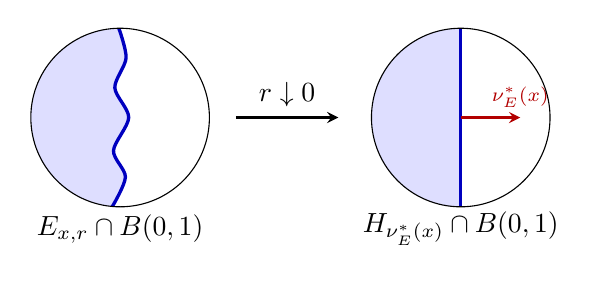
\begin{tikzpicture}[>=stealth,scale=0.84]
  \begin{scope}[shift={(0,0)}]
    \clip (0,0) circle (1.35);
    \fill[blue!13] (-1.5,-1.5)--(-0.10,-1.5)--(-0.12,-1.3)--
      (0.08,-0.9)--(-0.10,-0.5)--(0.13,0)--(-0.08,0.45)--
      (0.09,0.9)--(-0.02,1.5)--(-1.5,1.5)--cycle;
    \draw[blue!75!black,very thick] plot[smooth] coordinates
      {(-0.12,-1.35) (0.08,-0.9) (-0.10,-0.5) (0.13,0)
       (-0.08,0.45) (0.09,0.9) (-0.02,1.35)};
  \end{scope}
  \draw (0,0) circle (1.35);
  \node at (0,-1.68) {$E_{x,r}\cap B(0,1)$};
  \draw[->,thick] (1.75,0)--(3.3,0)
    node[pos=.5,above] {$r\downarrow0$};
  \begin{scope}[shift={(5.15,0)}]
    \clip (0,0) circle (1.35);
    \fill[blue!13] (-1.5,-1.5) rectangle (0,1.5);
    \draw[blue!75!black,very thick] (0,-1.4)--(0,1.4);
    \draw[->,red!70!black,thick] (0,0)--(0.9,0)
      node[above,font=\scriptsize] {$\nu_E^*(x)$};
  \end{scope}
  \draw (5.15,0) circle (1.35);
  \node at (5.15,-1.68) {$H_{\nu_E^*(x)}\cap B(0,1)$};
\end{tikzpicture}

\small\emph{Schemat granicy De Giorgiego:}
po przeskalowaniu przy punkcie brzegu zredukowanego
zbiór staje się półprzestrzenią w sensie zbieżności
$L^1_{\mathrm{loc}}$; rysunek nie oznacza zbieżności
brzegów w odległości Hausdorffa.
\end{center}

\begin{uwaga}[Brzeg topologiczny a zredukowany]
Twierdzenie nie orzeka, że $\partial E=\partial^*E$.
Zmiana $E$ na zbiorze $\lambda_n$-zerowym może
zupełnie zmienić jego brzeg topologiczny,
lecz nie zmienia $D\chi_E$, obwodu ani wzoru
Gaussa--Greena. W szczególności właściwą
miarą powierzchniową dla ogólnych zbiorów
skończonego obwodu jest
$\mathcal H^{n-1}\llcorner\partial^*E$.
\end{uwaga}

\begin{lemat}[Mierzalność obwodów poziomic]
\label{lem:BV-level-meas-auditVI}
Niech $\Omega\subseteq\mathbb R^n$ będzie otwarty,
a $u:\Omega\to\mathbb R$ mierzalna. Wówczas funkcja
$t\mapsto P(\{u>t\};\Omega)$ o wartościach
w $[0,+\infty]$ jest borelowska. Analogicznie
$t\mapsto P(\{u<-t\};\Omega)$ jest borelowska.
Nie zakładamy skończoności obwodów.
\end{lemat}
\begin{proof}
Wybierzmy przeliczalne wyczerpanie $\Omega$
zbiorami zwartymi $K_j\subset\operatorname{int}K_{j+1}$.
Dla każdego $j$ istnieje przeliczalna rodzina
pól $C_c^1(\Omega;\mathbb R^n)$ o nośnikach
w ustalonym otoczeniu $K_j$, gęsta w normie $C^1$
wśród pól testowych wspartych w $K_j$.
Można ją skonstruować z mollifikowanych funkcji
schodkowych na wymiernych siatkach, z wymiernymi
współczynnikami; następnie skalujemy pola, aby
ich normy punktowe nie przekraczały $1$.
Po złączeniu tych rodzin otrzymujemy ciąg
$(\varphi_j)$, dla którego
\[
 P(E;\Omega)=\sup_j\int_E
 \operatorname{div}\varphi_j(x)\,\mathrm d\lambda_n(x)
\]
dla każdego zbioru mierzalnego $E$; każdą całkę
wolno tu zastąpić jej wartością z przeciwnym znakiem,
bo rodzina pól jest symetryczna. Uzasadnieniem
równości jest aproksymacja w normie $C^1$
na wspólnym zwartym nośniku i ograniczoność
$\lambda_n$ na tym nośniku.
Dla ustalonego $j$ odwzorowanie
$t\mapsto\int_\Omega\chi_{\{u>t\}}(x)
\operatorname{div}\varphi_j(x)\,\mathrm d\lambda_n(x)$
jest borelowskie: funkcja
$(t,x)\mapsto\chi_{\{u(x)>t\}}\operatorname{div}\varphi_j(x)$
jest mierzalna i jest zdominowana przez
całkowalną funkcję $|\operatorname{div}\varphi_j|$.
Co więcej, powstała funkcja $t$ jest borelowska:
rozcinamy $\operatorname{div}\varphi_j$ na części dodatnią
i ujemną; każda z odpowiadających całek jest
niemalejąca przy $t\downarrow-\infty$ (czyli
nierosnąca jako funkcja $t$), więc jest borelowska.
Supremum przeliczalnie wielu funkcji
borelowskich jest borelowskie. Analogiczny
argument działa dla $\{u<-t\}$.
\end{proof}

\section{Współobszar, funkcje BV i warstwowanie}
\begin{twierdzenie}[Jedna nierówność formuły koobszaru dla $BV$]
\label{thm:BV-layercake-29}
Niech $\Omega\subseteq\mathbb R^n$ będzie otwarty,
$u\in L^1(\Omega)$, a dla prawie wszystkich $t>0$
zbiory $E_t^+=\{u>t\}$ i $E_t^-=\{u<-t\}$
mają skończony obwód w $\Omega$. Jeśli
\[
 \int_0^\infty\!P(E_t^+;\Omega)\,\mathrm d\lambda_1(t)
 +\int_0^\infty\!P(E_t^-;\Omega)\,\mathrm d\lambda_1(t)<\infty,
\]
to $u\in BV(\Omega)$ i
\[
 |Du|(\Omega)\le\int_0^\infty
 [P(E_t^+;\Omega)+P(E_t^-;\Omega)]\,
 \mathrm d\lambda_1(t).
\]
\end{twierdzenie}
\begin{proof}
Warstwowanie funkcji daje punktowo
$u(x)=\int_0^\infty[\chi_{\{u>t\}}(x)
-\chi_{\{u<-t\}}(x)]\,\mathrm dt$
poza zbiorem, na którym $u$ nie jest skończona.
Równość ma sens w $L^1(\Omega)$, gdyż
$\int_0^\infty\lambda_n(\{|u|>t\})\,\mathrm dt
=\int_\Omega|u(x)|\,\mathrm d\lambda_n(x)<\infty$.
Dla testowego pola $\varphi$ o $|\varphi|\le1$
możemy zastosować Fubiniego i otrzymujemy
\[
 \int_\Omega u(x)\operatorname{div}\varphi(x)
 \,\mathrm d\lambda_n(x)
 =\int_0^\infty\!\left(
 \int_{E_t^+}\operatorname{div}\varphi(x)
 \,\mathrm d\lambda_n(x)
 -\int_{E_t^-}\operatorname{div}\varphi(x)
 \,\mathrm d\lambda_n(x)\right)\mathrm dt.
\]
Z definicji obwodu wartość wyrażenia w nawiasie
jest nie większa niż
$P(E_t^+;\Omega)+P(E_t^-;\Omega)$.
Biorąc supremum po testach, otrzymujemy tezę.
\end{proof}

\section{Pełna formuła koobszaru dla funkcji $BV$}
Związek między obwodem zbiorów poziomic a wariacją
funkcji nie wymaga twierdzenia strukturalnego De Giorgiego.
Wystarczą ścisła aproksymacja w $BV$, gładki wzór
koobszaru z Rozdziału~\ref{ch:area-coarea-28} i dolna
półciągłość wariacji.

\begin{lemat}[Ścisła aproksymacja gładka w $BV$]
\label{lem:BV-strict-approx}
Niech $\Omega\subseteq\mathbb R^n$ będzie otwarty,
a $u\in BV(\Omega)$. Istnieją funkcje
$u_j\in C^\infty(\Omega)\cap W^{1,1}(\Omega)$ takie, że
\[
 \|u_j-u\|_{L^1(\Omega)}\longrightarrow0,
 \qquad
 \int_\Omega|\nabla u_j(x)|\,\mathrm d\lambda_n(x)
 \longrightarrow |Du|(\Omega).
\]
Nie wymaga się regularności brzegu $\Omega$.
\end{lemat}
\begin{proof}
Wybieramy lokalnie skończoną gładką partycję
jedności $(\psi_i)_{i\ge1}$ na $\Omega$,
$\psi_i\ge0$, $\psi_i\in C_c^\infty(\Omega)$,
$\sum_i\psi_i=1$. Można ją skonstruować z
przeliczalnego pokrycia $\Omega$ kulami o zwartych
domknięciach w $\Omega$: lokalnie skończone
funkcje odcinające normalizujemy ich sumą.
Niech $\rho_\varepsilon$ będzie nieujemnym
gładkim mollifikatorem o masie $1$.
Dla ustalonego $j$ wybieramy dodatnie
$\varepsilon_{i,j}$ tak małe, aby nośniki
$\rho_{\varepsilon_{i,j}}*(\psi_i u)$ mieściły
się w ustalonych lokalnie skończenie wielu
otoczeniach $\operatorname{supp}\psi_i$,
a ponadto
\begin{align*}
 \|\rho_{\varepsilon_{i,j}}*(\psi_i u)-\psi_i u\|_1
 &<2^{-i-j},\\
 \|\rho_{\varepsilon_{i,j}}*(u\nabla\psi_i)
              -u\nabla\psi_i\|_1
 &<2^{-i-j}.
\end{align*}
Wszystkie normy dotyczą $\mathbb R^n$ po
przedłużeniu funkcji o zwartej podporze przez $0$.
Możliwość wyboru wynika z ciągłości mollifikacji
w $L^1$; obydwa wyrażenia są całkowalne, ponieważ
$u\in L^1(\Omega)$, a $\psi_i$ ma zwarty nośnik.
Definiujemy
$u_j=\sum_i\rho_{\varepsilon_{i,j}}*(\psi_i u)$.
Suma jest lokalnie skończona i należy do
$C^\infty(\Omega)\cap L^1(\Omega)$, a z pierwszego
oszacowania
$\|u_j-u\|_1\le2^{-j}$.

Reguła Leibniza w sensie miar daje
$D(\psi_i u)=\psi_i Du+u\nabla\psi_i\,\lambda_n$:
wystarczy w definicji pochodnej dystrybucyjnej
podstawić pole testowe pomnożone przez $\psi_i$
i rozwinąć klasyczną pochodną iloczynu.
Dlatego
\[
 \nabla u_j
 =\sum_i\rho_{\varepsilon_{i,j}}*(\psi_i Du)
 +\sum_i\bigl[\rho_{\varepsilon_{i,j}}*(u\nabla\psi_i)
                  -u\nabla\psi_i\bigr],
\]
gdyż $\sum_i\nabla\psi_i=0$ lokalnie,
a więc $\sum_i u\nabla\psi_i=0$ prawie wszędzie.
Dla pierwszej sumy stosujemy nierówność trójkąta,
Tonellego i nieujemność $\psi_i$:
\[
 \int_\Omega\left|
 \sum_i\rho_{\varepsilon_{i,j}}*(\psi_i Du)(x)
 \right|\,\mathrm d\lambda_n(x)
 \le\sum_i\int_\Omega\psi_i(x)\,\mathrm d|Du|(x)
 =|Du|(\Omega).
\]
Druga suma ma normę $L^1$ co najwyżej $2^{-j}$.
Zatem $\int_\Omega|\nabla u_j(x)|\,\mathrm d\lambda_n(x)
\le|Du|(\Omega)+2^{-j}$, co jednocześnie dowodzi,
że $u_j\in W^{1,1}(\Omega)$.
Nierówność odwrotna dla granicy wynika z
dolnej półciągłości wariacji z
Twierdzenia~\ref{thm:perimeter-lsc-29}:
$|Du|(\Omega)\le\liminf_j\int_\Omega|\nabla u_j|$.
\end{proof}

\begin{lemat}[Obwody poziomic funkcji gładkiej]
\label{lem:BV-smooth-levels}
Jeżeli $v\in C^1(\Omega)$ i
$\int_\Omega|\nabla v(x)|\,\mathrm d\lambda_n(x)<\infty$,
to dla prawie każdego $t\in\mathbb R$
zbiór $\{v>t\}$ ma skończony obwód oraz
\[
 \int_{-\infty}^{\infty}P(\{v>t\};\Omega)
 \,\mathrm d\lambda_1(t)
 \le\int_\Omega|\nabla v(x)|\,\mathrm d\lambda_n(x).
\]
\end{lemat}
\begin{proof}
Wybierzmy gładką, niemalejącą funkcję
$\theta:\mathbb R\to[0,1]$, równą $0$ na
$(-\infty,0]$ i $1$ na $[1,\infty)$, i niech
$\theta_\varepsilon(s)=\theta(s/\varepsilon)$.
Dla pola $\varphi\in C_c^1(\Omega;\mathbb R^n)$
całkowanie przez części daje
\[
 \int_\Omega\theta_\varepsilon(v(x)-t)
 \operatorname{div}\varphi(x)\,\mathrm d\lambda_n(x)
 =-\int_\Omega\theta'_\varepsilon(v(x)-t)
 \nabla v(x)\cdot\varphi(x)\,\mathrm d\lambda_n(x).
\]
Dla prawie każdego $t$ zbiór $\{v=t\}$ ma
zerową miarę Lebesgue'a (możliwe wyjątki
są co najwyżej przeliczalne na wyczerpaniu
$\Omega$ zwartymi podzbiorami). Lewa strona
zbiega więc do $\int_{\{v>t\}}\operatorname{div}\varphi$.
Z kolei wzór koobszaru dla odwzorowania
$v:\Omega\to\mathbb R$ pozwala zapisać
prawą stronę jako
\[
 -\int_{\mathbb R}\theta'_\varepsilon(s-t)
 \left(\int_{\{v=s,\,\nabla v\ne0\}}
 \frac{\nabla v(x)}{|\nabla v(x)|}\cdot\varphi(x)
 \,\mathrm d\mathcal H^{n-1}(x)\right)
 \,\mathrm d\lambda_1(s).
\]
Funkcja w nawiasie należy do $L^1(\mathbb R)$,
ponieważ jej moduł jest ograniczony przez
$\|\varphi\|_\infty\mathcal H^{n-1}
(\{v=s,\nabla v\ne0\}\cap\operatorname{supp}\varphi)$,
a całka tej ostatniej wielkości jest skończona
na mocy koobszaru i całkowalności $|\nabla v|$.
Twierdzenie Lebesgue'a o różniczkowaniu daje
zatem dla prawie wszystkich $t$
\[
 \int_{\{v>t\}}\operatorname{div}\varphi(x)
 \,\mathrm d\lambda_n(x)
 =-\int_{\{v=t,\,\nabla v\ne0\}}
 \frac{\nabla v(x)}{|\nabla v(x)|}\cdot\varphi(x)
 \,\mathrm d\mathcal H^{n-1}(x).
\]
Wybierając przeliczalny zbiór pól testowych
gęsty w normie $C^1$ na zwartych nośnikach
i przechodząc do granicy, uzyskujemy powyższą
równość dla wszystkich pól testowych na
wspólnym zbiorze poziomów pełnej miary.
W szczególności
$P(\{v>t\};\Omega)\le
\mathcal H^{n-1}(\{v=t,\nabla v\ne0\})$.
Całkujemy po $t$ i ponownie stosujemy koobszar,
otrzymując tezę.
\end{proof}

\begin{twierdzenie}[Pełna formuła koobszaru dla $BV$]
\label{thm:BV-coarea-full-29}
Niech $\Omega\subseteq\mathbb R^n$ będzie otwarty.
Jeżeli $u\in BV(\Omega)$, to dla prawie wszystkich
$t\in\mathbb R$ zbiór $\{x\in\Omega:u(x)>t\}$
ma skończony obwód w $\Omega$ oraz
\begin{equation}\label{eq:BV-coarea-full-29}
 |Du|(\Omega)=\int_{-\infty}^{\infty}
 P(\{u>t\};\Omega)\,\mathrm d\lambda_1(t).
\end{equation}
W szczególności dla każdego $u\in BV_{\mathrm{loc}}(\Omega)$
i otwartego $V\subseteq\Omega$ zachodzi równość,
być może z dwiema stronami równymi $+\infty$,
\[
 |Du|(V)=\int_{-\infty}^{\infty}
 P(\{u>t\};V)\,\mathrm d\lambda_1(t).
\]
\end{twierdzenie}
\begin{proof}
Najpierw niech $u\in BV(\Omega)$.
Wybierzmy z Lematu~\ref{lem:BV-strict-approx}
ciąg $u_j\in C^\infty(\Omega)\cap W^{1,1}(\Omega)$
zbiegający do $u$ w $L^1$, ze zbieżnością
całek z gradientu do $|Du|(\Omega)$.
Przechodząc do podciągu możemy założyć,
że $\sum_j\|u_j-u\|_{L^1}<\infty$.
Tożsamość liczbowa
$\int_{\mathbb R}|\chi_{\{a>t\}}-
\chi_{\{b>t\}}|\,\mathrm d\lambda_1(t)=|a-b|$
i twierdzenie Tonellego dają
\[
 \int_{\mathbb R}\|\chi_{\{u_j>t\}}-
 \chi_{\{u>t\}}\|_{L^1(\Omega)}
 \,\mathrm d\lambda_1(t)=\|u_j-u\|_{L^1(\Omega)}.
\]
Stąd dla prawie wszystkich $t$ zachodzi
$\chi_{\{u_j>t\}}\to\chi_{\{u>t\}}$
w $L^1(\Omega)$. Półciągłość obwodu,
Lemat~\ref{lem:BV-level-meas-auditVI},
nierówność Fatou i Lemat~\ref{lem:BV-smooth-levels}
dają
\begin{align*}
 \int_{\mathbb R}P(\{u>t\};\Omega)\,
 \mathrm d\lambda_1(t)
 &\le\liminf_j\int_{\mathbb R}
 P(\{u_j>t\};\Omega)\,\mathrm d\lambda_1(t)\\
 &\le\liminf_j\int_\Omega|\nabla u_j(x)|
 \,\mathrm d\lambda_n(x)=|Du|(\Omega).
\end{align*}
W szczególności prawie wszystkie poziomice
mają skończony obwód.

Nierówność w przeciwną stronę wynika z
Twierdzenia~\ref{thm:BV-layercake-29}.
Istotnie, dla $t>0$ używamy poziomic $\{u>t\}$,
a dla $t<0$ ich dopełnień, które są równe
$\{u<-|t|\}$ z dokładnością do zbioru
$\lambda_n$-zerowego, poza co najwyżej
przeliczalną liczbą poziomów $t$.
Wynika to z faktu, że na przestrzeni o mierze
$\sigma$-skończonej tylko przeliczalnie
wiele rozłącznych poziomic $\{u=t\}$ może
mieć dodatnią miarę. Obwód dopełnienia jest
taki sam, zatem
$\int_{\mathbb R}P(\{u>t\};\Omega)\,\mathrm d\lambda_1(t)$
można zapisać jako sumę obydwu całek
z Twierdzenia~\ref{thm:BV-layercake-29}.
To kończy dowód równości.

Dla $u\in BV_{\mathrm{loc}}(\Omega)$ i otwartego
$V\subseteq\Omega$ wybieramy wyczerpanie $V$
przez rosnące zbiory otwarte $V_j$ o zwartych
domknięciach w $\Omega$. Na każdym $V_j$
funkcja $u$ jest całkowalna i ma skończoną
wariację; stosujemy właśnie udowodnioną równość.
Ponieważ $|Du|(V_j)\uparrow|Du|(V)$
i $P(\{u>t\};V_j)\uparrow P(\{u>t\};V)$,
twierdzenie o zbieżności monotonicznej pozwala
przejść do granicy.
\end{proof}

\begin{wniosek}[Wzór koobszaru z wagą]
\label{cor:BV-coarea-weighted-29}
Niech $u\in BV_{\mathrm{loc}}(\Omega)$.
Dla każdej borelowskiej $g:\Omega\to[0,+\infty]$
zachodzi
\[
 \int_\Omega g(x)\,\mathrm d|Du|(x)
 =\int_{\mathbb R}\left(\int_\Omega g(x)
 \,\mathrm d|D\chi_{\{u>t\}}|(x)\right)
 \,\mathrm d\lambda_1(t).
\]
\end{wniosek}
\begin{proof}
Dla zbioru otwartego $V\subseteq\Omega$
równość obu stron, z $g=\chi_V$, to druga
część Twierdzenia~\ref{thm:BV-coarea-full-29}.
Zatem miara $|Du|$ i miara zadana prawą
stroną są równe na zbiorach otwartych.
Rzeczywiście, ta druga jest miarą: addytywność
wynika z twierdzenia Tonellego i addytywności
miar $|D\chi_{\{u>t\}}|$. Mierzalność względem
$t$ dla zbiorów otwartych wynika z
Lematu~\ref{lem:BV-level-meas-auditVI}.
Dla pozostałych zbiorów borelowskich ustalamy
wyczerpanie $\Omega$ zbiorami otwartymi o zwartych
domknięciach i ograniczamy się do takich zbiorów.
Dla prawie wszystkich $t$ obwód na każdym z nich
jest skończony. Dlatego twierdzenie o klasie
monotonicznej, zastosowane do zbiorów otwartych
i różnic takich zbiorów, daje mierzalność
$t\mapsto|D\chi_{\{u>t\}}|(A)$ dla każdego
zbioru borelowskiego $A$. Przez wyczerpanie
otrzymujemy to dla całej $\Omega$.
Obie miary są regularne i zgadzają się na
zbiorach otwartych, zatem są równe na
zbiorach borelowskich. Aproksymacja
nieujemnej funkcji borelowskiej funkcjami
prostymi kończy dowód.
\end{proof}

\begin{przyklad}[Funkcja ze skokiem i formuła koobszaru]
Niech $\Omega=(-2,2)$ i $u=\chi_{(0,1)}$.
Wtedy $Du=\delta_0-\delta_1$ jako miara
ze znakiem, zatem $|Du|(\Omega)=2$.
Dla $0<t<1$ mamy $\{u>t\}=(0,1)$ i
$P(\{u>t\};\Omega)=2$. Dla pozostałych
$t$, poza nieistotnymi poziomami $0$ i $1$,
obwód poziomicy jest zerowy: zbiór jest
pusty albo równy $\Omega$. Stąd
$\int_{\mathbb R}P(\{u>t\};\Omega)
\,\mathrm d\lambda_1(t)=\int_0^1 2\,
\mathrm d\lambda_1(t)=2$, zgodnie z
Twierdzeniem~\ref{thm:BV-coarea-full-29}.
\end{przyklad}

\begin{przyklad}[Gęsta zmiana reprezentanta nie zmienia brzegu zredukowanego]
Dla $E=(0,1)^n\setminus\mathbb Q^n$
zachodzi $\chi_E=\chi_{(0,1)^n}$ prawie wszędzie.
Stąd $|D\chi_E|$ jest miarą powierzchniową
na ścianach sześcianu, a jego brzeg zredukowany
zgadza się z sumą wnętrz ścian, z dokładnością
do zbioru $\mathcal H^{n-1}$-zerowego.
Natomiast brzeg topologiczny $E$ zawiera
cały domknięty sześcian, ponieważ zarówno
$E$, jak i jego dopełnienie są gęste
wewnątrz $[0,1]^n$. To pokazuje, że
brzeg topologiczny nie może zastępować
$\partial^*E$ w twierdzeniu De Giorgiego.
\end{przyklad}

\section{Elementy teorii prądów}
\begin{definicja}[Prąd i jego brzeg]
\label{def:current-29}
Niech $\Omega\subseteq\mathbb R^n$ będzie otwarty.
\emph{Prądem wymiaru $k$} nazywamy ciągły
funkcjonał liniowy na przestrzeni $\mathcal D^k(\Omega)$
gładkich $k$-form o zwartym nośniku, wyposażonej
w zwykłą topologię funkcji testowych.
Jeśli $T$ jest prądem wymiaru $k\ge1$, jego
\emph{brzeg} definiujemy przez
$\partial T(\omega)=T(\mathrm d\omega)$
dla $\omega\in\mathcal D^{k-1}(\Omega)$.
\end{definicja}

\begin{lemat}[Brzeg brzegu znika]
\label{lem:current-boundary-square-29}
Dla każdego prądu $T$ wymiaru $k\ge2$ zachodzi
$\partial(\partial T)=0$.
\end{lemat}
\begin{proof}
Dla $\omega\in\mathcal D^{k-2}(\Omega)$ mamy
$\partial(\partial T)(\omega)=
\partial T(\mathrm d\omega)=T(\mathrm d^2\omega)=0$,
gdyż z definicji różniczki zewnętrznej
$\mathrm d^2=0$.
\end{proof}

\begin{przyklad}[Prąd zadany przez powierzchnię]
Niech $S$ będzie zorientowaną zwartą gładką
$k$-wymiarową podrozmaitością z brzegiem
w $\Omega$. Wówczas $T_S(\omega)=\int_S\omega$
jest prądem wymiaru $k$. Z twierdzenia Stokesa
wynika $\partial T_S=T_{\partial S}$. Właśnie
w tej postaci klasyczny rachunek na rozmaitościach
staje się szczególnym przypadkiem teorii prądów.
\end{przyklad}

\section{Podsumowanie zależności i dalsze kierunki}
W rozdziale otrzymaliśmy reprezentację pochodnych
$BV$ przez miary, półciągłość i zwartość obwodu,
miarową formułę Gaussa--Greena, twierdzenie strukturalne
De Giorgiego wraz z geometrycznym opisem brzegu
zredukowanego oraz pełną formułę koobszaru dla $BV$.
Dowód twierdzenia strukturalnego opierał się na
nierównościach izoperymetrycznych, zwartości w $BV$,
granicach zbiorów po przeskalowaniu i prostowalności
wyprowadzonej z lokalnej płaskości.
Dowód formuły koobszaru był niezależny od
tej struktury: wykorzystał ścisłą aproksymację
gładką i wzór koobszaru dla odwzorowań Lipschitzowskich.
Dalsze zagadnienia to m.in. dokładne przedstawiciele
funkcji $BV$, twierdzenia śladowe, łańcuchowe
oraz teoria powierzchni minimalnych.

\begin{uwaga}[Miary wektorowe w dalszym ciągu skryptu]
Dla $u\in BV(\Omega)$ miara $Du$ ma skończoną wariację
i jest szczególnym przypadkiem miary o wartościach
w przestrzeni Banacha, omawianej w
Rozdziale~\ref{ch:vector-measures-30}.
W przypadku $u\in BV_{\mathrm{loc}}(\Omega)$ jej wariacja
jest tylko lokalnie skończona; nie musimy wtedy otrzymać
skończonego wektora $Du(\Omega)$.
Rozdział 30 interpretuje rozkład polarny poprzez RNP
przestrzeni $\mathbb R^n$. Nie należy jednak utożsamiać
tego rozkładu z istnieniem gęstości $Du$ względem
miary Lebesgue'a.
\end{uwaga}
